\chapter{Optimizations}

Modern SAT solvers use many advanced optimizations and heuristics to improve the solving time.
However these are usually designed for general problem instances.
With additional knowledge about a specific problem we can try to come up with better heuristics which lead to decrease of solving time.

In this chapter we will describe several optimizations that we implemented and evaluated.
Some of these involve a simple change in output instance generation, others involve changes to the SAT solvers themselves.

\section{Merging operators}
\label{sec:merging-operators}
Since all operators in the \emph{Python} programming language are either unary or binary so are all the nodes in the created boolean circuit.
Writing an expressions such as \texttt{X = A \& B \& C \& D} will result in the boolean circuit shown in figure \ref{fig:bc-comp:a} since the \emph{and} operator is left-to-right associative.

A simple recursive algorithm can be used to walk over the boolean circuit in reverse topological order and merge such structures into a single $n$-ary node.
At each step, if one or both of the operands of some boolean operator node are nodes of the same type, they can be merged together to a single node.
After repeating this procedure for the whole tree we obtain the result shown in figure \ref{fig:bc-comp:b}.

We implemented such optimization in our library and modified the clause generation code to support arbitrary arities.
This is a simple optimization that can reduce the number of variables and clauses required to encode the given model as a SAT instance.
Next we describe a more advanced method that can optimize not just sequences of identical operators but arbitrary expressions.

\begin{figure}
\centering
\subbottom[Before merging]{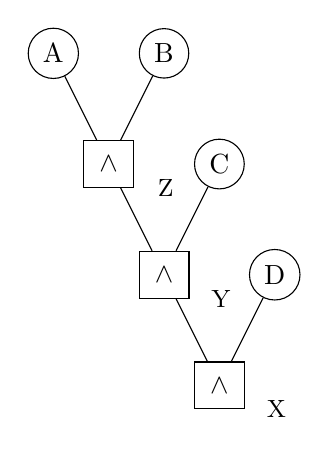
\begin{tikzpicture}[every node/.style = {draw, shape=rectangle, inner sep=2mm,},
             every tree node/.style={}, level distance=40pt, sibling distance=40pt]
\node (and1) {$\land$} [grow = up]
  child {node [shape=circle, inner sep=1mm] {D}}
  child {node (and2) {$\land$}
    child {node [shape=circle, inner sep=1mm] {C}}
    child {node (and3) {$\land$}
      child {node [shape=circle, inner sep=1mm] {B}}
      child {node [shape=circle, inner sep=1mm] {A}}
    }
  };

\node at (and1.south east) [xshift=4mm, draw=none] {\small X};
\node at (and2.south east) [xshift=4mm, draw=none] {\small Y};
\node at (and3.south east) [xshift=4mm, draw=none] {\small Z};
\end{tikzpicture}\label{fig:bc-comp:a}}
\hspace{2cm}
\subbottom[After merging]{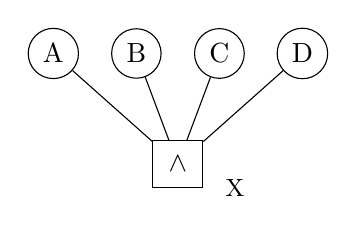
\begin{tikzpicture}[every node/.style = {draw, shape=rectangle, inner sep=2mm,},
             every tree node/.style={}, level distance=40pt, sibling distance=30pt]
\node (and1) {$\land$} [grow = up]
  child {node [shape=circle, inner sep=1mm] {D}}
  child {node [shape=circle, inner sep=1mm] {C}}
  child {node [shape=circle, inner sep=1mm] {B}}
  child {node [shape=circle, inner sep=1mm] {A}}
;

\node at (and1.south east) [xshift=4mm, draw=none] {\small X};
\end{tikzpicture}\label{fig:bc-comp:b}}
\caption{Comparing the effect of operator merging on the boolean circuit resulting from the expression \texttt{X = A \& B \& C \& D}.}
\end{figure}

\section{Expression encoding}
\label{sec:expression-encoding}
The automatic and transparent conversion from unmodified source code to SAT instance via operator overloading and boolean circuits may lead to suboptimal encoding of various expressions.
For example, the \emph{choice} round function in \emph{SHA-1}
\[
Ch(x, y, z) = (x \land y) \oplus (\overline{x} \land z)
\]
leads to an encoding with three variables and ten clauses (three clauses for each \emph{and} gate and four for the \emph{xor} gate) if we apply the Tseitin transformation directly:

% Naive Tseitin
% 1x 2y 3leftand 4notx 5z 6rightand 7result
%%%%%
%-3 1 0
%-3 2 0
%3 -1 -2 0
%4 1 0
%-4 -1 0
%-6 4 0
%-6 5 0
%6 -4 -5 0
%3 6 -7 0
%3 -6 7 0
%-3 6 7 0
%-3 -6 -7 0
\begin{align*}
(\overline{a} \lor x) \land (\overline{a} \lor y) \land (a \lor \overline{x} \lor \overline{y}) &~& \text{Left AND gate}\\
(\overline{b} \lor \overline{x}) \land (\overline{b} \lor z) \land (b \lor x \lor \overline{z})&~& \text{Right AND gate} \\
(c \lor a \lor \overline{b}) \land (c \lor \overline{a} \lor b) \land (\overline{c} \lor a \lor b) \land (\overline{c} \lor \overline{a} \lor \overline{b}) &~& \text{XOR gate}
\end{align*}

A better encoding using just six clauses and one variable is shown in \cite{nossum2012sat}:
\begin{align*}
&(\overline{a} \lor \overline{x} \lor y) \land (\overline{a} \lor x \lor z) \land (\overline{a} \lor y \lor z) \\
\land~ &(a \lor \overline{x} \lor \overline{y}) \land (a \lor x \lor \overline{z}) \land (a \lor \overline{y} \lor \overline{z})
\end{align*}

In fact, it is possible to encode this expression with just four clauses and one variable:
% Espresso opt
% 1x 2y 3z 4result
%%%%%
%-1 -2  4 0
%1 -3  4 0
%1 3  -4 0
%-1 2  -4 0
\begin{align*}
&(a \lor \overline{x} \lor \overline{y}) \land (a \lor x \lor \overline{z}) \land (\overline{a} \lor x \lor z) \land (\overline{a} \lor \overline{x} \lor y)
\end{align*}


%TODO move to section2 (library) after tseitin/boolean?
To solve this issue we provide an expression optimization function in our library.
Any $n$-ary expression can be wrapped using this function to replace the standard Tseitin encoding with a (potentially) smaller one, in terms of number of extra variables and clauses required.

\begin{minted}[linenos,
			   numbersep=5pt,
               frame=lines,
               framesep=2mm]{python}
# Unoptimized expression
f = (b & c) | (~b & d)

# Optimized using Espresso
choice = OptimizeExpression(lambda b, c, d: (b & c) | (~b & d))
f = choice(b, c, d)
\end{minted}


First we evaluate the expression on all $2^n$ possible inputs to generate a truth table.
It is then processed using an external truth table minimization tool \emph{Espresso} \cite{rudell1986multiple}, which generates a list of clauses that can be used to encode the expression.

When this expression is used anywhere in the model a node is created in the boolean circuit representation.
It behaves like any other node and can be used in further expressions, however during instance generation the optimized list of clauses is used instead of the na\"{\i}ve Tseitin encoding.

Using this optimization on the \emph{SHA-1} \emph{choice} round function does indeed lead to the minimal encoding with just four clauses as shown above.
Similarly, some steps of the \emph{SHA-3} hash function can be wrapped and optimized in this way.
Both of these optimizations are further described and evaluated in section \ref{sec:expression-encoding-eval}.

\section{Branching order}
\label{sec:branching-order}
%TODO nossum/soos mailing list cite; is it in text?; more references to literature

The most important heuristic in a SAT solver is the decision which unassigned variable to pick next.
A bad order might assign randomly picked values to many variables before some conflict is found and the search tree depth will be quite high.
This in turn leads to an increased solving time.
On the other hand a good heuristic would pick variables in an order that causes many propagations and with an unsatisfiable assignment leads to conflicts quickly.

The branching order is picked by a heuristic in the SAT solver, which does not have additional knowledge about what these variables represent and how they relate to each other.
By extending the input file format and the variable picking algorithm we can provide our own (partial) variable branching order.

\subsection{Implementation}
\label{sec:branching-order-impl}
We added a new input line type to the \emph{DIMACS CNF} file format.
A line in the form

\centerline{\texttt{b $v$ 0}}

\noindent means that variable $v$ should be branched on first.
When multiple such lines are provided the order of branching is the same as the order of these lines in the input file.
Using this we can provide a list of any number of variables in the order we want them to be picked for assignment.

We modified the popular \emph{MiniSat} solver \cite{een2005minisat} to be able to parse and store this list.
Then we modified the selection of next branching candidate to first pick all these variables in the specified order.
Once all have been assigned we fall back to the standard branching order algorithm.

We also made similar changes to the \emph{CryptoMiniSat} solver \cite{soos2009extending}, which is based on MiniSat.
However since we got better performance from using MiniSat only this solver was used for further evaluation.

We have also added support for this feature to our modeling library.
Before the boolean circuit is transformed to a set of CNF clauses and written to a file, the user can specify arbitrary branching order using variables defined in the model of the cryptographic primitive:

\begin{minted}[linenos,
			   numbersep=5pt,
               frame=lines,
               framesep=2mm]{python}
instance.assignVars(all_variables)

for var in variables_for_branching:
    instance.branch(var)

instance.emit(all_variables)
instance.solve(['minisat'])
\end{minted}